\chapter{Aplicação das regras de transição}

Após a otimização das regras de transição utilizando o EDA, nós avaliamos o desempenho das regras em classificar corretamente os elementos de estrutura secundária. A regra de transição que apresentou a melhor acurácia ao longo da evolução do EDA foi utilizada em um autômato celular determinístico, onde cada elemento da regra apresenta sempre a mesma transição.

Além do autômato celular determinístico, nós utilizamos as probabilidades da última geração do EDA como uma regra de transição para um autômato celular probabilístico. No autômato probabilístico, cada elemento da regra apresenta uma probabilidade de transitar para cada um dos estados existentes.

\section{Autômato celular determinístico}

A aplicação do autômato celular determinístico no conjunto de proteínas diversas resultou em um Q3 médio de 54.0\% com desvio padrão de 8.47. Quando analisamos a acurácia por elementos de estrutura secundária (Qh, Qe, Qc), notamos um alto índice de acerto na predição de hélices (Qh=74.7\%) em relação a coils (Qc=65.5\%) e sobretudo fitas (Qe=18.6\%). Isso é um indício de que o maior número de resíduos em hélices tem conduzido a predição à um excessivo número de hélices. Como mencionado anteriormente, acreditamos que será necessária a alteração da função de fitness para corrigir esse resultado.

\begin{figure}
	\centering
	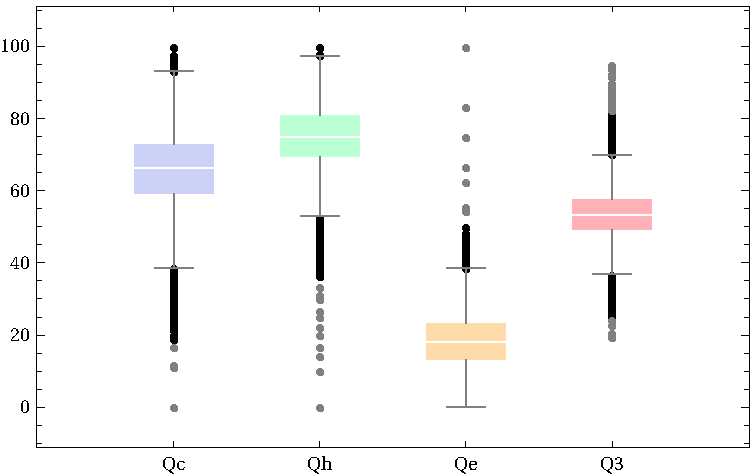
\includegraphics[width=0.9\textwidth]{figures/q3.pdf}
	\caption{q3}
	\label{fig:q3}
\end{figure}

Entretanto, avaliamos a capacidade preditiva do modelo utilizando também a curva ROC. A curva ROC de cada elemento da estrutura secundária permite avaliar como a frequência de cada estado durante a evolução do autômato celular está relacionada a estrutura correta. Assim, por exemplo, caso tivéssemos um valor de limiar qualquer para as frequências de hélice onde acima do limiar a estrutura secundária atribuída fosse uma hélice, a área sob a curva ROC (AUC) seria igual a 1. Caso o preditor fosse randômico teríamos uma AUC próxima a 0.5. 

A área sob a curva ROC nos fornece informação sobre como a frequência de estados de cada elemento de estrutura secundária comporta-se em relação a estrutura secundária atribuída. Os valores obtidos ($AUC > 0.7$) indica que as frequências tendem a possuir valores maiores para elementos de estrutura secundária corretos (Figuras \ref{fig:roc_coil}, \ref{fig:roc_helix} e \ref{fig:roc_strand}). Os resultados das curvas ROC nos mostram que mesmo a predição de fitas, que apresentou baixa acurácia, tende a apresentar frequências maiores dos estados de fita para os que são atribuídos a esse estado.   

\begin{figure}
	\centering
	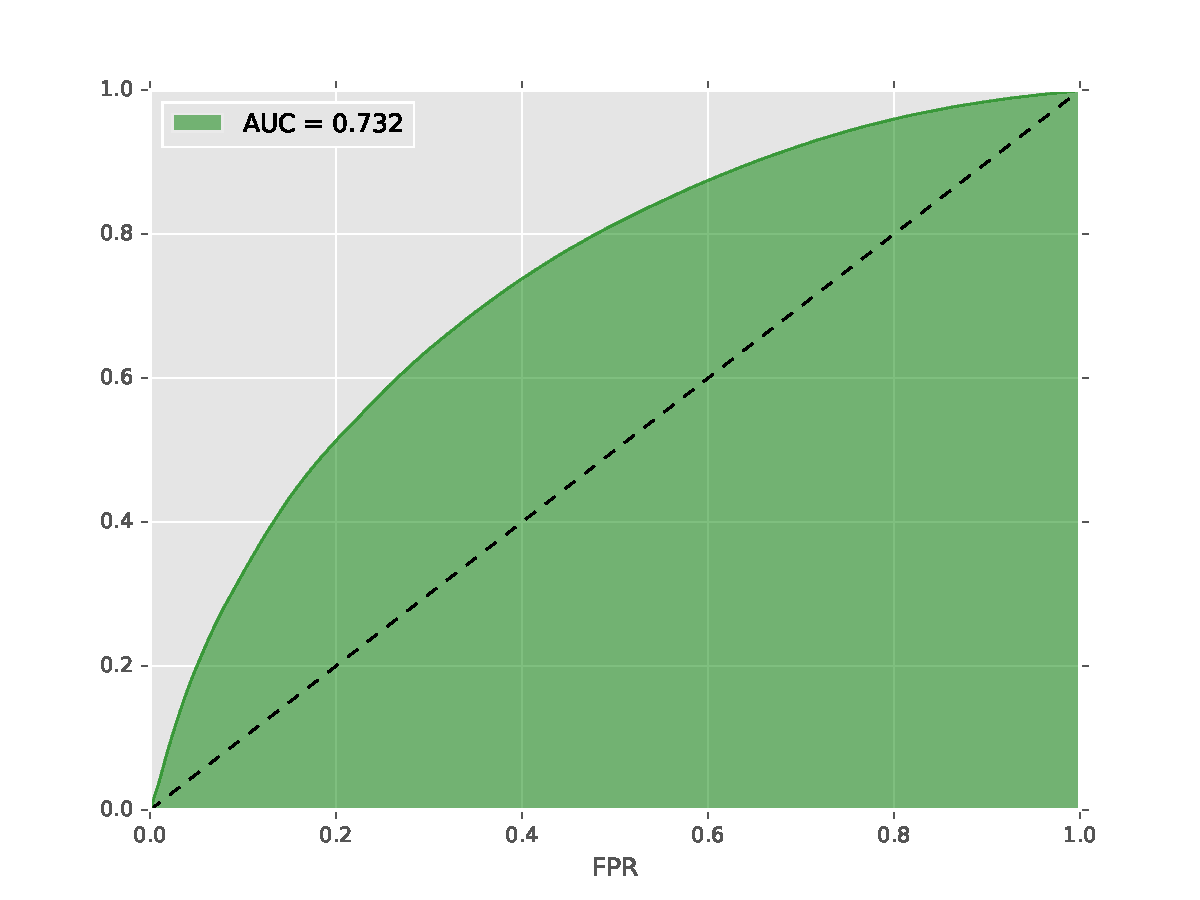
\includegraphics[width=0.9\textwidth]{figures/figure_roc_coil.pdf}
	\caption{Gráfico da curva ROC para coils contruído a partir dos resultados do CA determinístico.}
	\label{fig:roc_coil}
\end{figure}

\begin{figure}
	\centering
	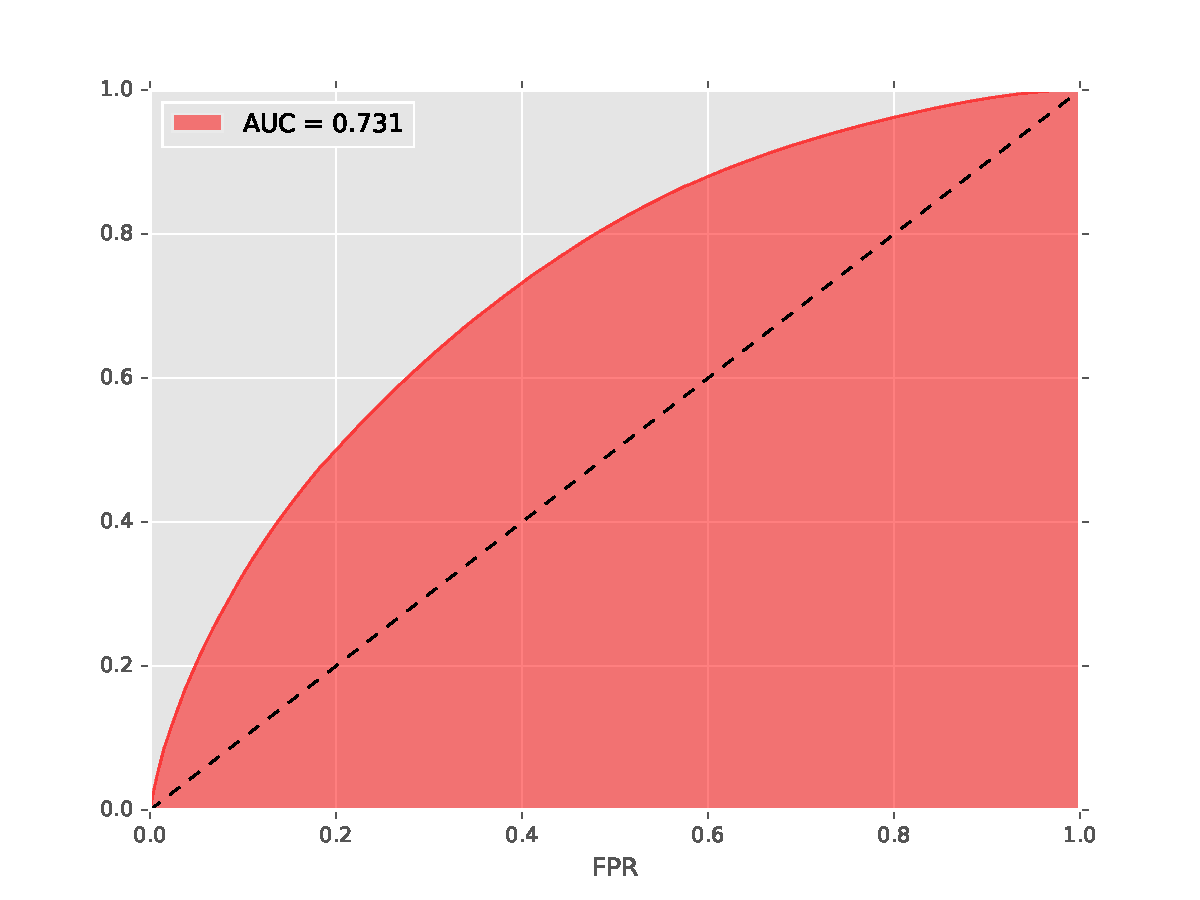
\includegraphics[width=0.9\textwidth]{figures/figure_roc_helix.pdf}
	\caption{Gráfico da curva ROC para hélices contruído a partir dos resultados do CA determinístico.}
	\label{fig:roc_helix}
\end{figure}

\begin{figure}
	\centering
	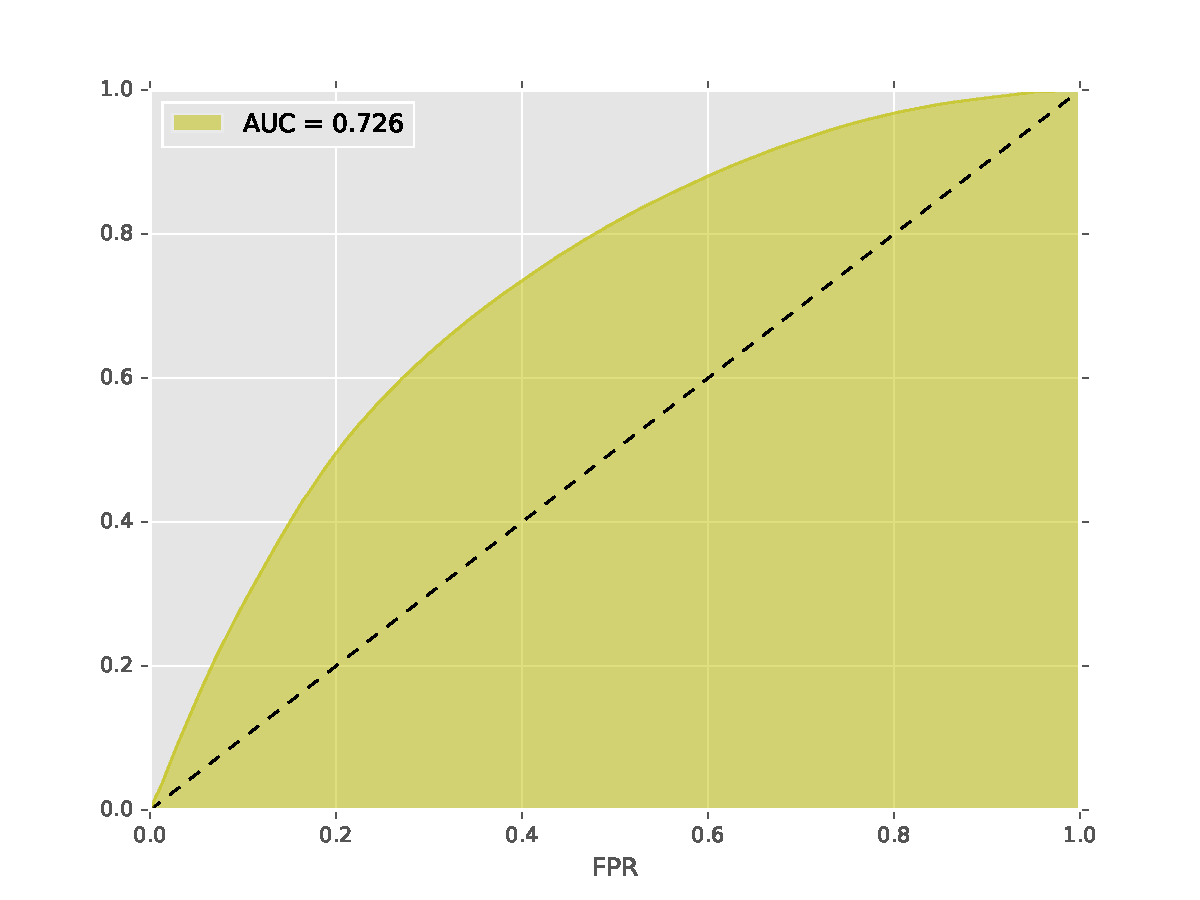
\includegraphics[width=0.9\textwidth]{figures/figure_roc_strand.pdf}
	\caption{Gráfico da curva ROC para fitas contruído a partir dos resultados do CA determinístico.}
	\label{fig:roc_strand}
\end{figure}



% Problema: Pode ser que esse não seja a melhor maneira de calcular a ROC para as 3 classes. Sugestão, calcular a ROC curve como a diferença entre o valor de hélice até o maior valor de frequencia, exceto hélice. Esse será o valor que será analisado. Comparar as ROC curves.    

% Outra forma de construirmos a curva ROC é utilizar a diferença entre a frequência do estado correto na evolução do autômato e a frequência do maior estado incorreto. Continuar a aplicação e inserir novas figuras de curva ROC 


\section{Autômato celular probabilístico}

O autômato celular probabilístico apresentou uma acurácia semelhante ao determinístico, com Q3 médio de 53.7\% e desvio padrão de 8.47. A acurácia para cada elemento de estrutura secundária (Qc, Qh, Qe)  apresentaram valores semelhantes ao CA determinístico, com a acurácia da predição de fitas muito inferior aos demais elementos. 


\begin{figure}
	\centering
	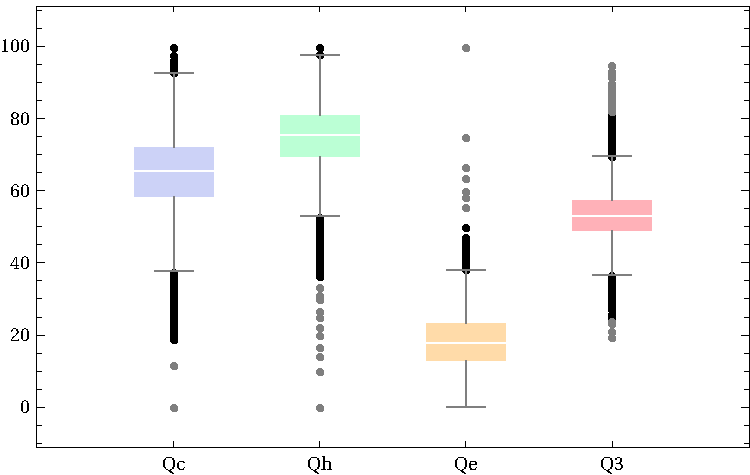
\includegraphics[width=0.9\textwidth]{figures/q3_prob.pdf}
	\caption{q3 prob}
	\label{fig:q3_prob}
\end{figure}


No CA probabilístico a área sob a curva ROC demonstrou que a frequência dos estados durante a evolução do CA apresenta relação com a estrutura secundária verdadeira semelhante à observada no CA determinístico (Figuras \ref{fig:roc_coil_prob}, \ref{fig:roc_helix_prob} e \ref{fig:roc_strand_prob}).  

\begin{figure}
	\centering
	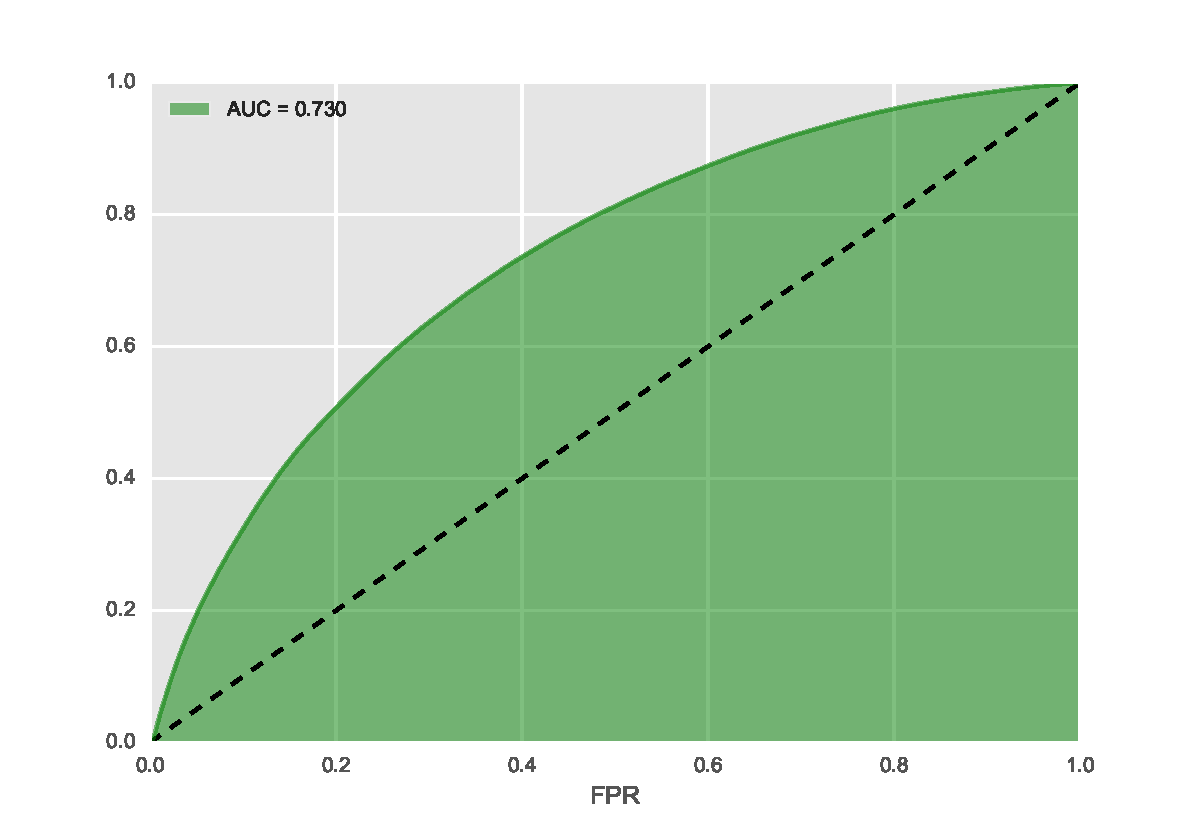
\includegraphics[width=0.9\textwidth]{figures/figure_roc_coil_prob.pdf}
	\caption{Gráfico da curva ROC para coils contruído a partir dos resultados do CA probabilístico.}
	\label{fig:roc_coil_prob}
\end{figure}

\begin{figure}
	\centering
	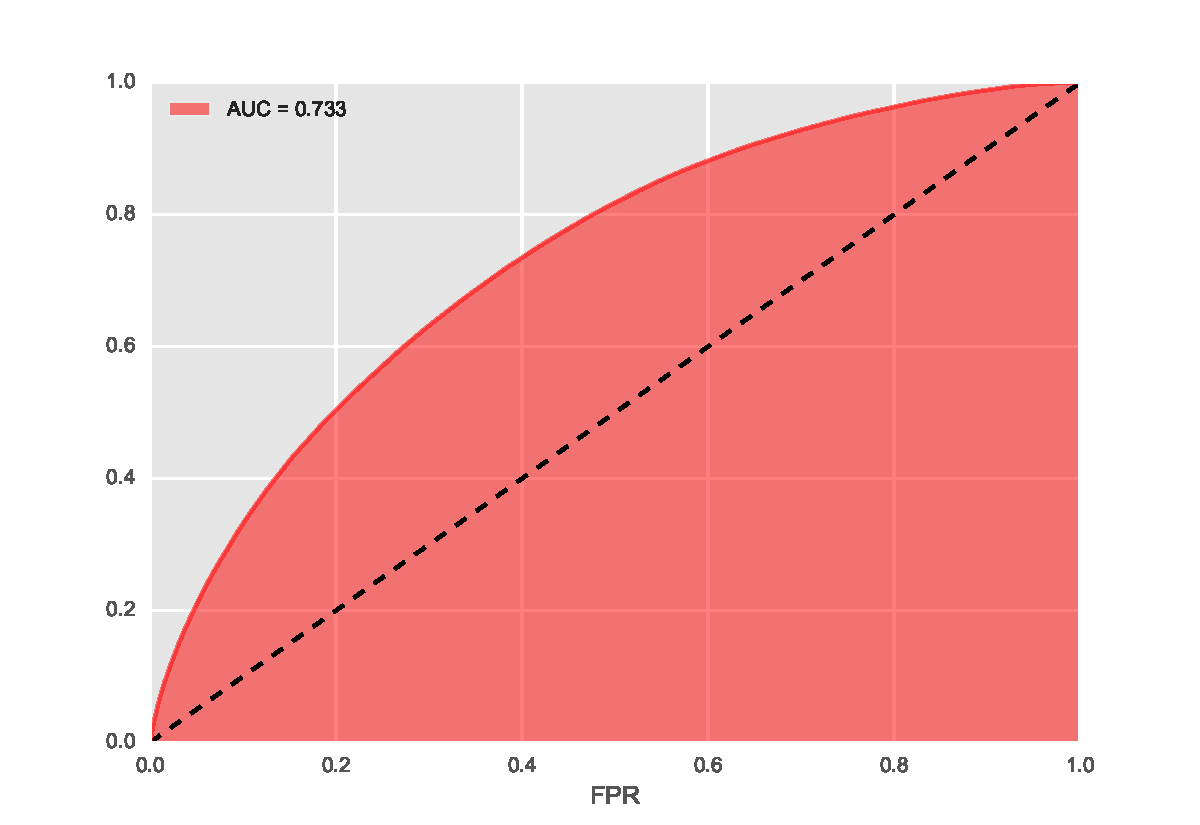
\includegraphics[width=0.9\textwidth]{figures/figure_roc_helix_prob.pdf}
	\caption{Gráfico da curva ROC para hélices contruído a partir dos resultados do CA probabilístico.}
	\label{fig:roc_helix_prob}
\end{figure}

\begin{figure}
	\centering
	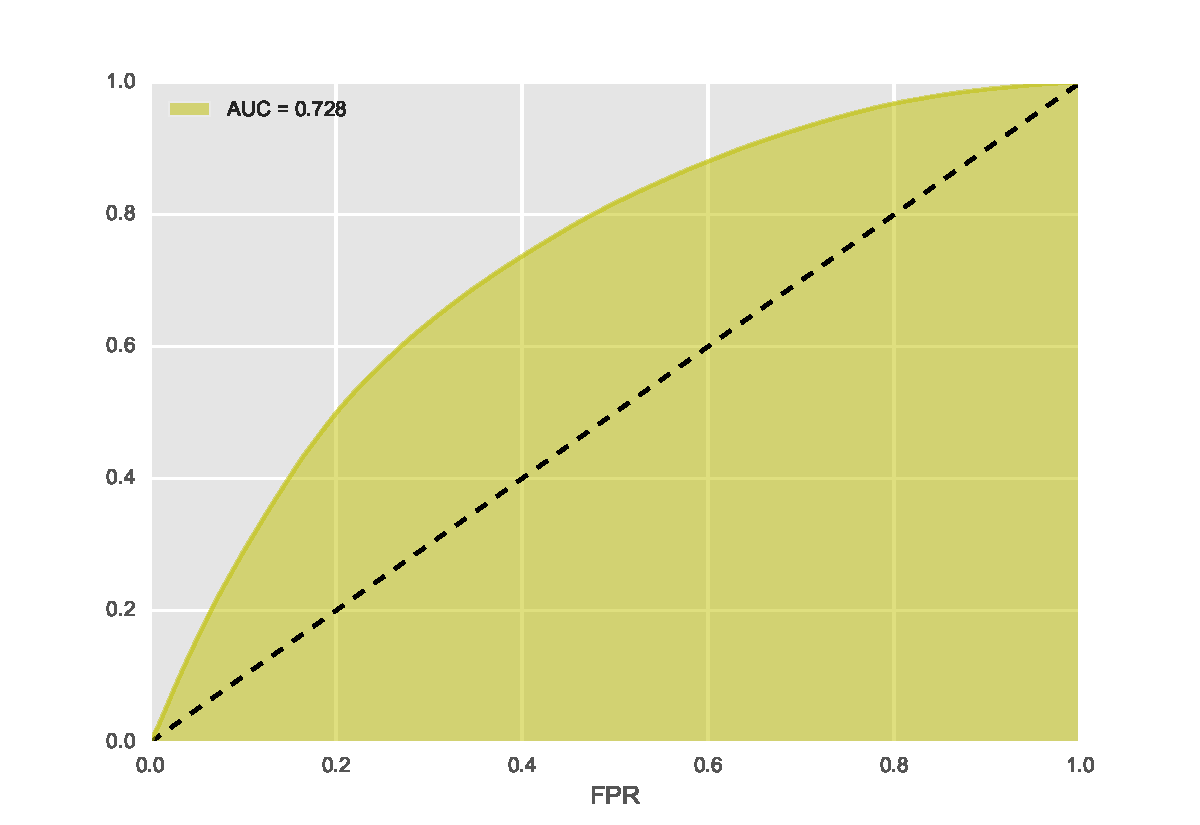
\includegraphics[width=0.9\textwidth]{figures/figure_roc_strand_prob.pdf}
	\caption{Gráfico da curva ROC para fitas contruído a partir dos resultados do CA probabilístico.}
	\label{fig:roc_strand_prob}
\end{figure}


\begin{table}
	\myfloatalign
	\begin{tabularx}{\textwidth}{Xcc} 
		\toprule
		 & \tableheadline{CA determinístico}  & \tableheadline{CA probabilístico} \\ 
%		\multicolumn{3}{c}{CA determinístico}  & \multicolumn{2}{c}{CA probabilístico} \\ 
		\midrule
		Q3 & 54.0 & 53.7 \\
		Qc & 65.5 & 64.9 \\
		Qh & 74.7 & 74.8 \\
		Qe & 18.6 & 18.4 \\
		AUCc & 0.732 & 0.730 \\
		AUCh & 0.731 & 0.733 \\
		AUCe & 0.726 & 0.728 \\
		\bottomrule
	\end{tabularx}
	\caption{Comparação entre a acurácia obtida utilizando os CAs determinístico e probabilístico. Ambos os CAs apresentam desempenho semelhante. }  \label{tab:q3_diff}
\end{table}




\section{Aplicação da regra de transição generalizada ao conjunto de proteínas com alta identidade sequencial e diferentes estruturas}


A proteína Ga98 e seus mutantes, os quais sofrem alterações globais na estrutura secundária, são casos interessantes para o teste de novas metodologias de predição de estrutura secundária. Nas metodologias atuais, que comumente utilizam redes neurais, a predição é feita utilizando uma janela de resíduos, em geral com comprimentos de 9, 11 ou 13 resíduos, onde o resíduo central da janela é classificado pela rede neural. Como a predição nas demais janelas presentes na sequência polipeptídica não influencia na classificação da janela, o método apresenta a limitação de responder apenas localmente às variações dos dados de entrada.  

Por outro lado, os autômatos celulares, apesar de evoluírem de acordo com regras locais, tem a capacidade de propagar as variações locais e influenciar o surgimento ou alteração de padrões globais, distantes do ponto de origem da variação. 

Para avaliar a capacidade dos modelos propostos e da eficácia do método de otimização em encontrar regras capazes de reproduzir o padrão correspondente às estruturas secundárias, testamos as regras de transição otimizadas para o conjunto de proteínas diversas.


